%        File: arfc-beamer.tex
%     Created: Sun May 5 10:00 PM 2013 C
%


%\documentclass[11pt,handout]{beamer}
\documentclass[9pt]{beamer}
\usetheme[white]{Illinois}
%\title[short title]{long title}
\title[ORNL Internship Progress Report]{ }
%\subtitle[short subtitle]{long subtitle}
\subtitle[Progress Report]{Progress Report}
%\author[short name]{long name}
\author[Jin Whan Bae]{Jin Whan Bae}
%\date[short date]{long date}
\date[05.21.2018 (week 2)]{June 06, 2018 (week 2)}
%\institution[short name]{long name}
\institute[UIUC]{University of Illinois at Urbana-Champaign}

%%%% Acronym support

\usepackage[acronym,toc]{glossaries}
\newacronym{NNL}{NNL}{National Nuclear Laboratory}
\newacronym{MA}{MA}{minor actinide}
\newacronym{DU}{DU}{depleted uranium}
\newacronym{LWR}{LWR}{Light Water Reactor}
\newacronym{MOX}{MOX}{Mixed Oxide Fuel}
\newacronym{SFR}{SFR}{Sodium-cooled Fast Reactor}
\newacronym{FLM}{FLM}{Fuel Loading Model}
\newacronym{EFMC}{EFMC}{Effective fissile mass coefficient}
\newacronym{ORNL}{ORNL}{Oak Ridge National Laboratory}
\newacronym{PWR}{PWR}{Pressurized Water Reactor}
\newacronym{FIT}{FIT}{Functionality Isolation Test}

\makeglossaries

%\usepackage{bbding}
\usepackage{amsfonts}
\usepackage{lipsum}
\usepackage{adjustbox}
\usepackage{fancyvrb}
\usepackage{amsmath}
\usepackage{xspace}
\usepackage{graphicx}
\usepackage{subfigure}
\usepackage{listings}
\usepackage{booktabs} % nice rules for tables
\usepackage{microtype} % if using PDF
\usepackage{bigints}
\DeclareMathOperator{\erf}{erf}
%I need some complimentary error funcitons... 
\DeclareMathOperator{\erfc}{erfc}
%page numbers
\setbeamertemplate{footline}[page number]
\setbeamertemplate{caption}[numbered]
%Those icons in the references are terrible looking
\setbeamertemplate{bibliography item}[text]


%try to get rid of header on title page\dots
\makeatletter
    \newenvironment{withoutheadline}{
        \setbeamertemplate{headline}[default]
        \def\beamer@entrycode{\vspace*{-\headheight}}
    }{}
\makeatother



\newcommand\blfootnote[1]{%
  \begingroup
  \renewcommand\thefootnote{}\footnote{#1}%
  \addtocounter{footnote}{-1}%
  \endgroup
}

\usepackage{booktabs} % nice rules (thick lines) for tables
\usepackage{microtype} % improves typography for PDF
\usepackage{xspace}
\usepackage{tabularx}
\usepackage[affil-it]{authblk}
\usepackage{tikz}

\usepackage{tikz}
\usetikzlibrary{positioning, arrows, decorations, shapes}

\usetikzlibrary{shapes.geometric,arrows}
\tikzstyle{process} = [rectangle, rounded corners, minimum width=3cm, minimum height=1cm,text centered, draw=black, fill=blue!30]
\tikzstyle{object} = [ellipse, rounded corners, minimum width=3cm, minimum height=1cm,text centered, draw=black, fill=green!30]
\tikzstyle{arrow} = [thick,->,>=stealth]

\usepackage{cleveref}
\usepackage{datatool}
\newcolumntype{b}{X}
\newcolumntype{s}{>{\hsize=.5\hsize}X}
\newcolumntype{m}{>{\hsize=.75\hsize}X}

\newcommand{\Cyclus}{\textsc{Cyclus}\xspace}%
\graphicspath{ {images/} }
\usetikzlibrary{positioning, arrows, decorations, shapes }

\begin{document}
%%%%%%%%%%%%%%%%%%%%%%%%%%%%%%%%%%%%%%%%%%%%%%%%%%%%%%%%%%%%%
%% From uw-beamer Here's a handy bit of code to place at 
%% the beginning of your presentation (after \begin{document}):
\newcommand*{\alphabet}{ABCDEFGHIJKLMNOPQRSTUVWXYZabcdefghijklmnopqrstuvwxyz}
\newlength{\highlightheight}
\newlength{\highlightdepth}
\newlength{\highlightmargin}
\setlength{\highlightmargin}{2pt}
\settoheight{\highlightheight}{\alphabet}
\settodepth{\highlightdepth}{\alphabet}
\addtolength{\highlightheight}{\highlightmargin}
\addtolength{\highlightdepth}{\highlightmargin}
\addtolength{\highlightheight}{\highlightdepth}
\newcommand*{\Highlight}{\rlap{\textcolor{HighlightBackground}{\rule[-\highlightdepth]{\linewidth}{\highlightheight}}}}
%%%%%%%%%%%%%%%%%%%%%%%%%%%%%%%%%%%%%%%%%%%%%%%%%%%%%%%%%%%%%
%%--------------------------------%%
\begin{withoutheadline}
\frame{
  \titlepage
}
\end{withoutheadline}

%%--------------------------------%%

\section{Done}

\begin{frame}
    \frametitle{Cyclus Benchmark with ORION, VISION, DYMOND and MARKAL}
    from paper \textbf{Standardized Verification of Fuel Cycle Modeling}
    \begin{figure}[htbp!]
        \begin{center}
                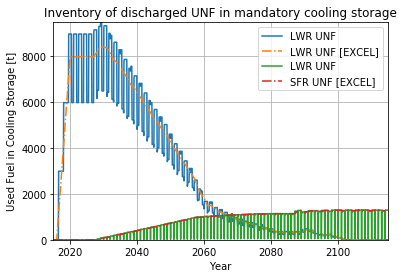
\includegraphics[width=.7\textwidth]{./images/verification/fuel_discharge_monthly.png}
        \end{center}
    \end{figure}

\end{frame}


\begin{frame}
    \frametitle{Cyclus Benchmark with ORION, VISION, DYMOND and MARKAL}
    from paper \textbf{Standardized Verification of Fuel Cycle Modeling}
    \begin{figure}[htbp!]
        \begin{center}
                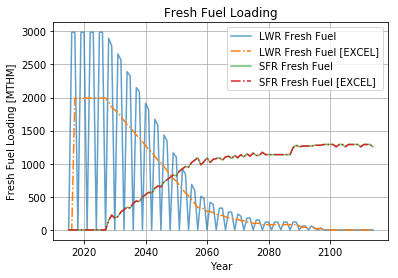
\includegraphics[width=.7\textwidth]{./images/verification/fuel_load.png}
        \end{center}
    \end{figure}

\end{frame}



\begin{frame}
    \frametitle{Cyclus Benchmark with ORION, VISION, DYMOND and MARKAL}
    from paper \textbf{Standardized Verification of Fuel Cycle Modeling}
    \begin{figure}[htbp!]
        \begin{center}
                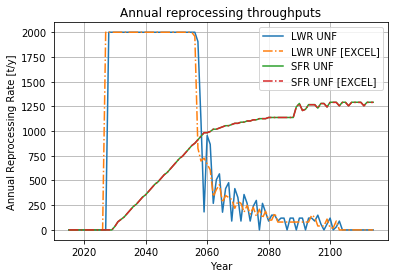
\includegraphics[width=.7\textwidth]{./images/verification/rep.png}
        \end{center}
    \end{figure}

\end{frame}



\begin{frame}
    \frametitle{Cyclus Benchmark with ORION, VISION, DYMOND and MARKAL}
    from paper \textbf{Standardized Verification of Fuel Cycle Modeling}
    \begin{figure}[htbp!]
        \begin{center}
                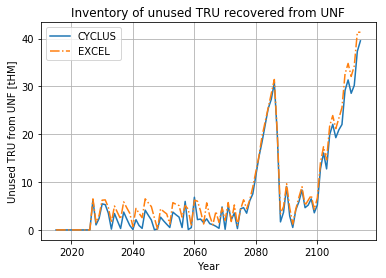
\includegraphics[width=.7\textwidth]{./images/verification/tru.png}
        \end{center}
    \end{figure}

\end{frame}


\begin{frame}
    \frametitle{Cyclus Benchmark with ORION, VISION, DYMOND and MARKAL}
    from paper \textbf{Standardized Verification of Fuel Cycle Modeling}
    \begin{figure}[htbp!]
        \begin{center}
                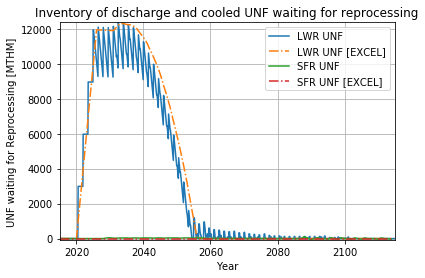
\includegraphics[width=.7\textwidth]{./images/verification/waiting_monthly.png}
        \end{center}
    \end{figure}

\end{frame}

\section{Doing}

\begin{frame}
    \frametitle{UDB data comparison}
    Compare UNF inventory between UDB data vs average enrichment / burnup data.
    Currently done with recipe (average burnup / enrichment). UDB data simulation
    running (50\% done)
\end{frame}

\begin{frame}
    \frametitle{Transmutation Data}
    Use transmutation data to model transition scenario. Currently working on EG01-EG23
        \begin{figure}[htbp!]
        \begin{center}
                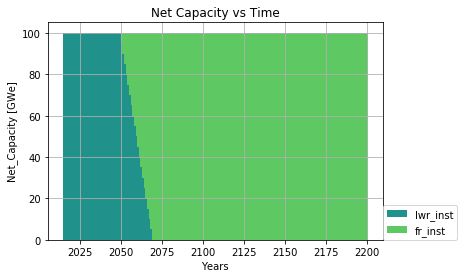
\includegraphics[width=.7\textwidth]{./images/transition/power_plot.png}
        \end{center}
    \end{figure}
\end{frame}

\begin{frame}
    \frametitle{Transmutation Data}
    Use transmutation data to model transition scenario. Currently working on EG01-EG23
        \begin{figure}[htbp!]
        \begin{center}
                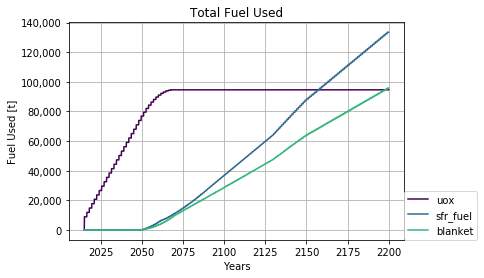
\includegraphics[width=.7\textwidth]{./images/transition/blanket_fuel.png}
        \end{center}
    \end{figure}
\end{frame}

\section{Dream}

\begin{frame}
    \frametitle{Regional Advanced Reactors in US}
    Various advanced reactors to meet regional demand in the U.S (desalination, process heat, hydrogen production, medical isotope production etc.)
\end{frame}

\begin{frame}
    \frametitle{Multiple-type fleet transition}
    Instead of EG01-EG23, try EG01-(EG23 + EG24 ...) something mixture where the 
    advanced reactors have some synergistic effect
\end{frame}

\begin{frame}
    \frametitle{MSR modling for fuel cycle}
    Recipe reactors won't cut it. ROM reactor module or using SCALE.
\end{frame}

\end{document}



